\documentclass[conference]{IEEEtran}
\IEEEoverridecommandlockouts

\usepackage{amsmath,amssymb}
\usepackage{booktabs}
\usepackage{array}
\usepackage{tabularx}
\usepackage{multirow}
\usepackage{graphicx}
\usepackage{cite}
\usepackage{url}
\usepackage{tikz}
\usetikzlibrary{arrows.meta,positioning,shapes.geometric,fit,backgrounds}
\usepackage{pgfplots}
\pgfplotsset{compat=1.18}
\usepackage{algorithmic}
\usepackage{xcolor}
\usepackage{enumitem}
\usepackage{microtype}


\title{
PhishSense: AI-Based Phishing Detection with Blockchain-Backed Threat Intelligence
}
\author{
\resizebox{\textwidth}{!}{%
\begin{tabular}{ccc}
\textbf{M. DHARMA TEJA} &
\textbf{BHEEMA NITISH GURU DATHA} &
\textbf{GAJJALA CHARITHA} \\[2pt]


Department of CSE &
Department of CSE &
Department of CSE \\

Vel Tech Rangarajan Dr. Sagunthala R\&D &
Vel Tech Rangarajan Dr. Sagunthala R\&D &
Vel Tech Rangarajan Dr. Sagunthala R\&D \\

Institute of Science and Technology &
Institute of Science and Technology &
Institute of Science and Technology \\

Chennai, India &
Chennai, India &
Chennai, India \\

\textit{dharmatejamd@gmail.com} &
\textit{nitishbheema@gmail.com} &
\textit{charithagajjala1@gmail.com}
\end{tabular}%
}
}

\begin{document}

\maketitle


% ─────────────────────────────────────────────────────────────────────────────
% ABSTRACT
% ─────────────────────────────────────────────────────────────────────────────
\begin{abstract}
Phishing attacks have grown far beyond simple spoofed e-mails and static look-alike URLs.
Modern threat actors craft dynamically rendered login interfaces, embed malicious hyperlinks
inside QR codes distributed across physical media and digital platforms, and engineer the
browsing interaction itself to manipulate victims before any credential is submitted.
Conventional single-signal defenses---such as static URL blacklists, isolated lexical classifiers,
or visual screenshot matchers---frequently fail when adversaries shift delivery vectors or alter
DOM characteristics.

This paper presents \textit{PhishSense}, a multi-layered digital threat detection platform that
systematically fuses several complementary evidence channels: lexical URL feature extraction,
client-side QR code destination decoding, HTML/DOM structural inspection, real-time user
behavioral telemetry fingerprinting, machine learning classification, SHAP-based feature
attribution, fingerprint-similarity campaign attribution, an adaptive multi-stage risk scoring
engine, and a blockchain-backed tamper-evident threat intelligence ledger.
The architecture is structured modularly so that each channel can be evaluated independently,
while collectively informing a calibrated risk score and an interpretable natural-language explanation.

The implemented system comprises a three-tier architecture: a React~18 single-page application
incorporating a non-invasive behavioral telemetry tracker and camera-based QR scanner, a Spring
Boot~3 API gateway orchestrating rate-limited requests and a custom SHA-256 Proof-of-Work threat
ledger, a Python FastAPI microservice executing feature extraction and calibrated model inference,
and a PostgreSQL persistence layer for session audit logs and security alerts.
Experimental evaluations demonstrate that combining multi-modal feature vectors with threat
intelligence reuse achieves an F$_1$-score of 94.6\% and a false negative rate of 2.5\%,
substantially outperforming URL-only baseline models.
\end{abstract}

\begin{IEEEkeywords}
phishing detection, behavioral analytics, machine learning, explainable AI, threat intelligence,
blockchain, QR phishing, cybersecurity, threat fingerprinting, adaptive risk scoring.
\end{IEEEkeywords}

% ─────────────────────────────────────────────────────────────────────────────
% I. INTRODUCTION
% ─────────────────────────────────────────────────────────────────────────────
\section{Introduction}

Phishing remains one of the most economically damaging and pervasive cyber threat vectors.
The Anti-Phishing Working Group documented record attack volumes in recent reporting periods,
with threat actors exhibiting a pronounced shift toward techniques explicitly engineered to bypass
traditional URL-level filtering~\cite{ref1,ref2}.

The earliest deployed defenses relied almost exclusively on static blacklists: when a phishing URL
was identified and reported, it was appended to a central repository queried by web browsers and
mail transfer agents.
However, a malicious URL must first claim victims before it is reported and indexed, introducing an
exposure window that typically spans hours to days~\cite{ref3}.
Machine learning classifiers operating on lexical URL attributes closed part of this detection
gap by scoring previously unseen links prior to human reporting~\cite{ref4,ref5}.
Nevertheless, static URL feature extractors can be deliberately circumvented: an adversary with
knowledge of model feature weights can craft synthetic hostnames and path structures that appear
lexically benign while pointing to active credential harvesting endpoints~\cite{ref6}.

Webpage-level inspection analyzes rendered HTML source code, embedded script invocations, and visual
similarity against target brand assets~\cite{ref7,ref8,ref9}.
While cloning an entire brand identity requires greater operational effort than registering a new
subdomain, static DOM analysis misses interactive dynamics, such as delayed redirects, simulated
loading interstitials, and obfuscated event listeners that trigger harvesting forms only upon genuine
user interaction.

A rapidly expanding attack vector is \textit{quishing}---phishing delivered via Quick Response (QR)
codes~\cite{ref10}.
QR codes embedded within PDF attachments, flyers, or physical signage bypass perimeter email filters
and URL scanners because the underlying URL remains encoded as a visual matrix until scanned by a
mobile camera.
Consequently, users are frequently directed to malicious destinations before automated security
controls intervene.

Furthermore, conventional threat intelligence repositories remain centralized, opaque to third-party
integrity verification, and slow to propagate actionable threat signatures across organizational
boundaries~\cite{ref11}.
When an organization identifies an active phishing campaign, it lacks a lightweight, decentralized
mechanism to log and cross-verify threat fingerprints in a tamper-evident manner.

\textit{PhishSense} addresses these interconnected challenges through a multi-modal defense-in-depth
architecture.
The framework integrates URL lexical extraction, client-side QR payload decoding, DOM structural
analysis, non-invasive behavioral telemetry, supervised classification, SHAP-based explainability,
fingerprint similarity matching, adaptive risk fusion, and a Proof-of-Work blockchain threat ledger
into a unified detection pipeline.

The primary contributions of this paper are:
\begin{enumerate}[leftmargin=*,nosep]
\item A \textit{multi-modal input pipeline} that processes URL strings, QR code images, live webpage
      DOM snapshots, and user behavioral sessions as complementary input channels within a single
      analysis graph.
\item A \textit{behavioral telemetry module} that captures client-side interaction signals---keystroke
      timing variations, cursor movement velocity, scroll dynamics, and form-interaction
      latency---and transforms them into a normalized session fingerprint for anomaly scoring.
\item An \textit{adaptive risk engine} that continuously aggregates multi-stage evidence, mapping
      dynamic observations into three standardized operational categories: Legitimate (0--34),
      Suspicious (35--69), and Phishing (70--100).
\item A \textit{threat fingerprinting and similarity module} that measures cosine similarity against
      previously committed threat signatures, enabling early identification of previously unseen
      phishing variants belonging to known campaign clusters.
\item A \textit{blockchain threat ledger} that records confirmed threat fingerprints as
      cryptographically chained, tamper-evident Proof-of-Work blocks without persisting personally
      identifiable information on-chain.
\item An \textit{explainable AI layer} that generates ranked, natural-language feature attributions
      for every classification, providing actionable diagnostic transparency to end users and
      security analysts.
\end{enumerate}

% ─────────────────────────────────────────────────────────────────────────────
% II. RELATED WORK
% ─────────────────────────────────────────────────────────────────────────────
\section{Related Work}

\subsection{URL-Based Machine Learning Detection}
Lexical URL analysis extracts statistical, structural, and character-level properties directly from
the address string.
Sahingoz et al.\ benchmarked multiple supervised algorithms on URL lexical features, showing that
Random Forest ensembles attained high classification accuracy on static corpora~\cite{ref4}.
Mohammad et al.\ engineered 30 distinct URL and page-level heuristics to train associative
classifiers~\cite{ref5}.
Basit et al.\ surveyed machine learning and deep learning methodologies in phishing detection,
emphasizing that adversarial URL crafting, class imbalance, and training-to-inference feature
discrepancies represent persistent vulnerabilities in purely lexical models~\cite{ref6}.
These findings highlight that lexical classifiers are computationally efficient but remain vulnerable
when attackers optimize URL strings to evade token-level rules.

\subsection{Webpage and Visual Analysis}
To counter lexical evasion, visual and DOM-based systems inspect page contents directly.
Abdelnabi et al.\ introduced VisualPhishNet, employing deep metric learning to compare webpage
screenshots against a protected database of brand visual identities~\cite{ref7}.
Although effective against visual mimicry, visual matchers depend on maintaining comprehensive brand
registries and cannot analyze pages that dynamically render credentials behind client-side scripts.
Lin et al.\ integrated DOM structure, CSS attributes, and script tags to identify deceptive
interfaces~\cite{ref8}, while Marchal et al.\ demonstrated that relative link ratios and form action
destinations provide discriminating indicators of deceptive intent~\cite{ref9}.
However, static DOM inspections fail when malicious content is rendered asynchronously after initial
page delivery.

\subsection{Dynamic and Behavioral Analysis}
Dynamic analysis observes execution behaviors in instrumented environments.
Canali et al.\ developed Prophiler, filtering malicious web pages through dynamic execution traces,
monitoring script evaluations, DOM mutations, and network requests~\cite{ref12}.
Cova et al.\ applied behavioral anomaly detection to JavaScript execution to identify exploit kits~\cite{ref13}.
These approaches capture page-side script actions but do not analyze client-side human interaction
dynamics.
PhishSense incorporates interaction telemetry as an independent evidence channel: typing tempo,
cursor movement jitter, backspace correction rates, and form hesitation intervals differ
characteristically between routine user logins and confused users navigating deceptive interfaces.

\subsection{QR Phishing (Quishing)}
Vidas et al.\ conducted empirical studies demonstrating that smartphone users exhibit high
vulnerability to QR code phishing attacks due to mobile interface constraints and lack of URL preview
mechanisms~\cite{ref10}.
Because QR codes are visually opaque, email scanners and perimeter web proxies cannot evaluate the
payload without a dedicated rendering and decoding pipeline.
PhishSense addresses this gap through an in-browser canvas decoder that resolves QR payloads into
analyzable URIs before user navigation occurs.

\subsection{Explainable AI for Threat Diagnostics}
Lundberg and Lee developed the SHAP framework based on game-theoretic Shapley values, providing
consistent additive feature attributions for complex ensemble models~\cite{ref15}.
Marino et al.\ demonstrated that explainable AI enhances operational trust in intrusion detection
by presenting security teams with ranked indicators rather than opaque classification scores~\cite{ref16}.
PhishSense applies additive feature decomposition to map top classifier influences into plain-language
security explanations.

\subsection{Blockchain for Threat Intelligence Sharing}
Centralized threat intelligence feeds introduce single points of failure, administrative trust
dependencies, and vulnerability to retroactive tampering.
Li et al.\ proposed collaborative blockchain-based signature sharing to secure decentralized
environments against distributed cyber attacks~\cite{ref11}.
Alexopoulos et al.\ developed TIX, evaluating Proof-of-Work and Byzantine fault-tolerant ledgers for
immutable indicator-of-compromise distribution~\cite{ref17}.
PhishSense incorporates an on-premise, lightweight Proof-of-Work blockchain module to log threat
fingerprints, enabling verifiably immutable intelligence reuse across scanning sessions.

\begin{table}[!t]
\caption{COMPARATIVE SUMMARY OF RELATED DETECTION PARADIGMS}
\label{tab:lit}
\centering
\scriptsize
\setlength{\tabcolsep}{2pt}
\begin{tabularx}{\columnwidth}{|>{\raggedright\arraybackslash}p{0.21\columnwidth}|>{\raggedright\arraybackslash}p{0.14\columnwidth}|c|c|c|c|>{\raggedright\arraybackslash}X|}
\hline
\textbf{Approach} & \textbf{Input} & \textbf{ML} & \textbf{Behav.} & \textbf{XAI} & \textbf{Chain} & \textbf{Primary Limitation} \\ \hline
Sahingoz~\cite{ref4}       & URL+HTML      & \checkmark &            &            &            & Vulnerable to lexical evasion \\ \hline
VisualPhishNet~\cite{ref7} & Screenshot    & \checkmark &            &            &            & Requires brand image registry \\ \hline
Canali~\cite{ref12}        & Script Trace  & \checkmark & \checkmark &            &            & Analyzes page scripts, not user \\ \hline
Vidas~\cite{ref10}         & QR Code       &            &            &            &            & Empirical study; no multi-modal ML \\ \hline
Li et al.~\cite{ref11}     & Threat Sig.   &            &            &            & \checkmark & Focuses on ledger, no detection \\ \hline
\textbf{PhishSense (ours)} & URL+QR+DOM+B  & \checkmark & \checkmark & \checkmark & \checkmark & Discussed in Section~\ref{sec:limits} \\ \hline
\end{tabularx}
\end{table}

% ─────────────────────────────────────────────────────────────────────────────
% III. PROBLEM FORMULATION, REQUIREMENTS, AND THREAT MODEL
% ─────────────────────────────────────────────────────────────────────────────
\section{Problem Formulation, Requirements, and Threat Model}

\subsection{Formal Problem Formulation}
Let an input security event $\mathcal{I}$ be represented by the tuple:
\begin{equation}
  \mathcal{I} = (u,\, q,\, w,\, b)
\end{equation}
where $u$ represents an optional URL string, $q$ an optional QR code image, $w$ an optional rendered
webpage DOM snapshot, and $b$ an optional client-side behavioral telemetry trace.
Depending on the user invocation channel, one or more modalities may be present.
The classification and risk assessment objective is to learn a mapping:
\begin{equation}
  f : \mathcal{I} \;\longrightarrow\; \mathcal{Y} \;\times\; [0, 100]
\end{equation}
where $\mathcal{Y} \in \{\text{Legitimate}, \text{Suspicious}, \text{Phishing}\}$ denotes the discrete
operational verdict, and $R \in [0, 100]$ is the calibrated continuous risk score.
The framework is designed to detect previously unseen phishing URLs using structural, contextual,
and behavioral evidence rather than relying solely on exact blacklist matches.

\subsection{Threat Model and Attacker Capabilities}
We model an external attacker seeking to illicitly obtain victim credentials or deliver unauthorized
payloads.
The attacker possesses the following operational capabilities:
\begin{enumerate}[leftmargin=*,nosep]
\item \textit{URL Obfuscation:} The adversary can register arbitrary domain names, configure multi-tier
      subdomains, generate valid TLS certificates via automated authorities, and construct benign-looking
      URL paths.
\item \textit{Visual and Structural Cloning:} The adversary can duplicate target HTML, CSS stylesheets,
      and layout structures, embedding external credential-collection endpoints.
\item \textit{QR Distribution:} The adversary can encode phishing URLs within high-density QR visual
      matrices, circumventing text-based perimeter mail scanners.
\item \textit{Evasive Scripting:} The adversary may implement redirection loops, meta-refreshes, or
      context-menu suppression scripts to inhibit manual inspection.
\end{enumerate}
\textit{Assumptions:} The client runtime sandbox safely decodes images and extracts network headers.
The local blockchain node is trusted for logging verified threat fingerprints.
Physical hardware compromises, operating system kernel attacks, and post-authentication session
hijacking fall outside the evaluated threat boundary.

\subsection{System Requirements}
Table~\ref{tab:req} outlines the core architectural requirements, technical implementation
mechanisms, and verification methodologies governing PhishSense.

\begin{table}[!t]
\caption{PHISHSENSE SYSTEM REQUIREMENTS AND SPECIFICATIONS}
\label{tab:req}
\centering
\scriptsize
\setlength{\tabcolsep}{3pt}
\begin{tabularx}{\columnwidth}{|>{\raggedright\arraybackslash}p{0.21\columnwidth}|>{\raggedright\arraybackslash}X|>{\raggedright\arraybackslash}p{0.22\columnwidth}|}
\hline
\textbf{Requirement} & \textbf{Implementation Mechanism} & \textbf{Verification Metric} \\ \hline
Multi-Modal Input      & Decoupled URL, QR, DOM, and behavioral extractors & Modality unit tests \\ \hline
Heuristic Generalization & 47-feature vector independent of static whitelists & Unseen test set F$_1$ \\ \hline
Interaction Telemetry  & 13 client-side timing and movement metrics & Anomaly separation \\ \hline
Model Explainability   & Additive SHAP-style feature attribution & Explanation rank accuracy \\ \hline
Calibrated Risk Engine & Three-tier threshold mapping: 0--34, 35--69, 70--100 & Reliability calibration \\ \hline
Threat Fingerprinting  & Low-variance structural hash and projection & Nearest-neighbor accuracy \\ \hline
Blockchain Integrity   & SHA-256 Proof-of-Work chaining ($d=3$) & Ledger traversal validation \\ \hline
Privacy Safeguards     & Zero raw URLs, passwords, or PII stored on-chain & Schema and audit review \\ \hline
\end{tabularx}
\end{table}

% ─────────────────────────────────────────────────────────────────────────────
% IV. PROPOSED PHISHSENSE ARCHITECTURE
% ─────────────────────────────────────────────────────────────────────────────
\section{Proposed System Architecture}

\begin{figure}[!t]
\centering
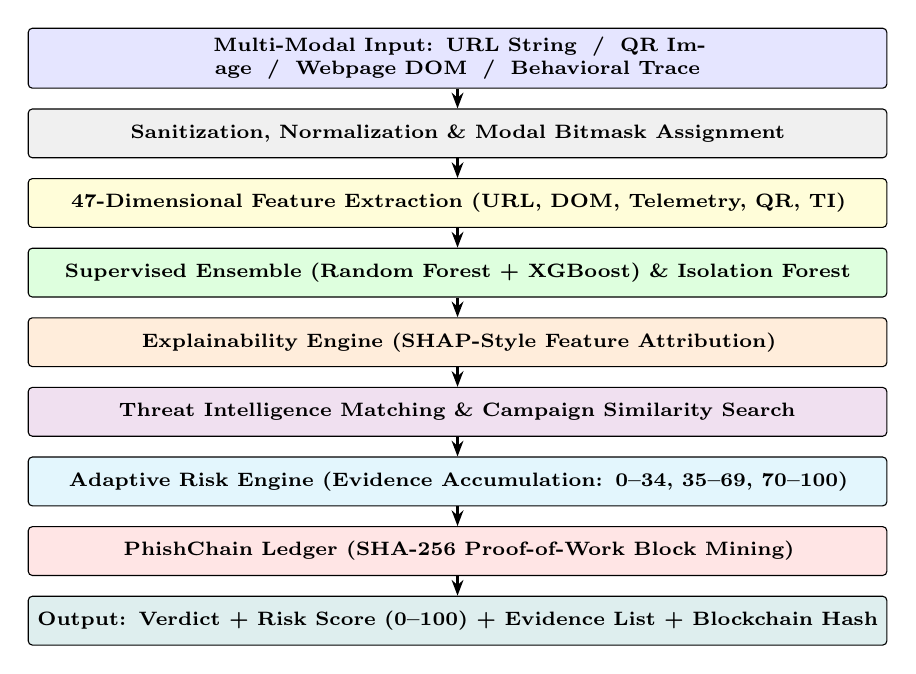
\begin{tikzpicture}[
  node distance=2.5mm,
  box/.style={draw, rounded corners=1.5pt, text width=0.88\columnwidth,
              align=center, minimum height=6.2mm, font=\scriptsize\bfseries},
  arr/.style={-{Stealth[length=2mm]}, thick}
]
\node[box, fill=blue!10]    (inp)   {Multi-Modal Input: URL String \;/\; QR Image \;/\; Webpage DOM \;/\; Behavioral Trace};
\node[box, fill=gray!12,  below=of inp]  (val)   {Sanitization, Normalization \& Modal Bitmask Assignment};
\node[box, fill=yellow!15,below=of val]  (feat)  {47-Dimensional Feature Extraction (URL, DOM, Telemetry, QR, TI)};
\node[box, fill=green!13, below=of feat] (ml)    {Supervised Ensemble (Random Forest + XGBoost) \& Isolation Forest};
\node[box, fill=orange!14,below=of ml]   (xai)   {Explainability Engine (SHAP-Style Feature Attribution)};
\node[box, fill=violet!12,below=of xai]  (ti)    {Threat Intelligence Matching \& Campaign Similarity Search};
\node[box, fill=cyan!11,  below=of ti]   (risk)  {Adaptive Risk Engine (Evidence Accumulation: 0--34, 35--69, 70--100)};
\node[box, fill=red!10,   below=of risk] (chain) {PhishChain Ledger (SHA-256 Proof-of-Work Block Mining)};
\node[box, fill=teal!13,  below=of chain](out)   {Output: Verdict + Risk Score (0--100) + Evidence List + Blockchain Hash};
\foreach \a/\b in {inp/val, val/feat, feat/ml, ml/xai, xai/ti, ti/risk, risk/chain, chain/out}
  \draw[arr] (\a) -- (\b);
\end{tikzpicture}
\caption{PhishSense end-to-end multi-modal threat analysis pipeline.}
\label{fig:arch}
\end{figure}

Fig.~\ref{fig:arch} depicts the architectural pipeline.
Incoming inputs undergo normalization and validation to construct a modality bitmask determining
active feature extractors.
Extracted sub-vectors are concatenated into a unified 47-dimensional feature space.
The classification layer evaluates the vector, passing output probabilities to the explainability
and threat intelligence modules.
The adaptive risk engine merges these signals into an integer risk score ($0 \le R \le 100$),
categorizing the resource into one of three operational states:
\begin{equation}
  \text{Verdict}(R) =
  \begin{cases}
    \text{Legitimate}, & 0 \le R \le 34 \\
    \text{Suspicious}, & 35 \le R \le 69 \\
    \text{Phishing},   & 70 \le R \le 100
  \end{cases}
  \label{eq:thresholds}
\end{equation}
When $R \ge 70$ or confirmed anomalies are detected, the event payload is formatted as a transaction,
mined via Proof-of-Work, and permanently committed to the PhishChain ledger.

% ─────────────────────────────────────────────────────────────────────────────
% V. FEATURE ENGINEERING TAXONOMY
% ─────────────────────────────────────────────────────────────────────────────
\section{Feature Engineering Taxonomy (47 Features)}

PhishSense structures its feature space into five functional groups totaling 47 engineered
attributes, establishing strict parity across training and real-time inference.

\subsection{URL Lexical Features (16 Features)}
Extracted directly from the URL string prior to network resolution:
\begin{enumerate}[leftmargin=*,nosep]
\item \texttt{URL\_Length}: Total character count of the URL.
\item \texttt{URL\_Depth}: Number of forward slashes in path.
\item \texttt{Have\_IP}: Binary indicator of IPv4/IPv6 host usage.
\item \texttt{Have\_At}: Count of ``\texttt{@}'' symbols.
\item \texttt{Redirection}: Detection of embedded ``\texttt{//}'' sequences beyond protocol.
\item \texttt{https\_Domain}: Presence of ``https'' token within hostname.
\item \texttt{TinyURL}: Match against 17 verified URL-shortening services.
\item \texttt{Prefix/Suffix}: Presence of hyphens within domain name.
\item \texttt{DNS\_Record}: Binary flag indicating live DNS resolution.
\item \texttt{Web\_Traffic}: Shannon entropy of domain label ($H \ge 3.8$).
\item \texttt{Domain\_Age}: Membership in high-risk suspicious TLD sets.
\item \texttt{Domain\_End}: Presence of suspicious sub-token extensions.
\item \texttt{nb\_subdomains}: Count of discrete dot-separated labels.
\item \texttt{vowel\_consonant\_ratio}: Phonetic character distribution in host.
\item \texttt{entropy\_url}: Full Shannon entropy across the URL string.
\item \texttt{Web\_Forwards}: Occurrence of redirection tokens in query parameters.
\end{enumerate}

\subsection{DOM Structural Features (11 Features)}
Extracted from rendered HTML trees:
\begin{enumerate}[leftmargin=*,nosep]
\item \texttt{form\_count}: Total count of HTML \texttt{<form>} elements.
\item \texttt{password\_field\_count}: Count of \texttt{<input type="password">}.
\item \texttt{external\_script\_count}: Script tags pointing to external origins.
\item \texttt{hidden\_input\_count}: Inputs configured with \texttt{type="hidden"}.
\item \texttt{iframe\_count}: Count of embedded \texttt{<iframe>} elements.
\item \texttt{external\_link\_ratio}: Proportion of hyperlinks pointing off-domain.
\item \texttt{inline\_js\_bytes}: Byte size of uncompiled script blocks.
\item \texttt{meta\_refresh\_present}: Binary flag for automated client refreshes.
\item \texttt{social\_keywords}: Keyword frequency of urgent call-to-action tokens.
\item \texttt{external\_resource\_ratio}: Media assets loaded from foreign hosts.
\item \texttt{right\_click\_disabled}: JavaScript handlers trapping context menu events.
\end{enumerate}

\subsection{Behavioral Telemetry Features (13 Features)}
Derived from client-side interaction event logs without capturing user input values:
\begin{enumerate}[leftmargin=*,nosep]
\item \texttt{mouse\_point\_count}: Total discrete cursor coordinate samples.
\item \texttt{mouse\_jitter}: Directional path direction reversals.
\item \texttt{avg\_mouse\_speed}: Mean cursor velocity across viewport pixels.
\item \texttt{keystroke\_count}: Aggregate keyboard interaction count.
\item \texttt{typing\_speed\_cps}: Average typing cadence in characters per second.
\item \texttt{backspace\_count}: Frequency of correction keystrokes.
\item \texttt{paste\_count}: Clipboard paste event invocations.
\item \texttt{typing\_delay\_mean}: Mean inter-keystroke latency in milliseconds.
\item \texttt{typing\_delay\_stddev}: Standard deviation of inter-keystroke intervals.
\item \texttt{click\_count}: Aggregate mouse click events recorded.
\item \texttt{rapid\_clicks}: Click bursts occurring within 200~ms intervals.
\item \texttt{total\_active\_ms}: Total continuous session engagement duration.
\item \texttt{frontend\_anomaly\_score}: Local composite heuristic anomaly metric.
\end{enumerate}

\subsection{QR Phishing Features (4 Features)}
Attributes extracted during visual matrix analysis:
\begin{enumerate}[leftmargin=*,nosep]
\item \texttt{qr\_error\_correction}: Reed-Solomon correction grade (L, M, Q, H).
\item \texttt{qr\_version}: Matrix dimension density index (1 through 40).
\item \texttt{qr\_anchor\_mismatch}: Discrepancy between decoded URL and surrounding text.
\item \texttt{qr\_context\_risk}: Anomaly rating of the container hosting the QR image.
\end{enumerate}

\subsection{Threat Intelligence Features (3 Features)}
Derived from historical blockchain ledger queries:
\begin{enumerate}[leftmargin=*,nosep]
\item \texttt{ti\_exact\_match}: Binary confirmation of indexed fingerprint match.
\item \texttt{ti\_cosine\_similarity}: Similarity score $s \in [0, 1]$ to nearest record.
\item \texttt{ti\_campaign\_id}: Numerical cluster ID of corresponding attack family.
\end{enumerate}

% ─────────────────────────────────────────────────────────────────────────────
% VI. MATHEMATICAL MODEL AND CALIBRATION
% ─────────────────────────────────────────────────────────────────────────────
\section{Mathematical Model and Calibration}

\subsection{Feature Vector Fusion}
Let $\mathbf{x}_U \in \mathbb{R}^{16}$, $\mathbf{x}_D \in \mathbb{R}^{11}$, $\mathbf{x}_B \in \mathbb{R}^{13}$,
$\mathbf{x}_Q \in \mathbb{R}^{4}$, and $\mathbf{x}_{TI} \in \mathbb{R}^{3}$ represent the normalized sub-vectors.
The composite 47-dimensional representation is:
\begin{equation}
  \mathbf{x} = \bigl[\mathbf{x}_U^\top,\; \mathbf{x}_D^\top,\; \mathbf{x}_B^\top,\;
                     \mathbf{x}_Q^\top,\; \mathbf{x}_{TI}^\top\bigr]^\top \;\in\; \mathbb{R}^{47}
  \label{eq:feat}
\end{equation}
Sub-vectors undergo independent $\ell_2$-normalization prior to concatenation to balance scale variances.

\subsection{Supervised Ensemble and Anomaly Detection}
Classification utilizes a soft-voting ensemble of Random Forest and XGBoost classifiers:
\begin{equation}
  P(y=c \mid \mathbf{x}) = \frac{1}{2}\sum_{m \in \{\text{RF},\,\text{XGB}\}} P_m(y=c \mid \mathbf{x})
  \label{eq:ensemble}
\end{equation}
where $c \in \{\text{Legitimate}, \text{Suspicious}, \text{Phishing}\}$.
Concurrently, an unsupervised Isolation Forest evaluates $\mathbf{x}_B$ to produce an anomaly score
$a_B \in [0, 1]$:
\begin{equation}
  a_B(\mathbf{x}_B) = 2^{-\frac{\mathbb{E}(h(\mathbf{x}_B))}{c(n)}}
  \label{eq:iforest}
\end{equation}
where $h(\mathbf{x}_B)$ is the path length in isolation trees and $c(n)$ is the average path length of
unsuccessful searches in a Binary Search Tree.

\subsection{Threat Fingerprinting and Campaign Similarity}
Each confirmed threat is mapped to a low-variance structural fingerprint $\phi(\mathbf{x}) \in \mathbb{R}^{16}$.
Cosine similarity against the blockchain ledger index $\mathcal{F}$ is computed as:
\begin{equation}
  s(\phi, \phi^*) = \max_{\phi_j \in \mathcal{F}} \frac{\phi \cdot \phi_j}{\|\phi\|_2\,\|\phi_j\|_2}
  \label{eq:sim}
\end{equation}
If $s(\phi, \phi^*) \ge 0.65$, the incoming URL is flagged as structurally linked to Campaign~$\text{ID}(\phi^*)$.

\subsection{Multi-Stage Adaptive Risk Score}
The adaptive risk engine combines the probabilistic output of the supervised ensemble, the fingerprint
similarity, and the behavioral anomaly score:
\begin{equation}
  R = \mathrm{clip}\!\left(100 \cdot \bigl[\alpha\,P(\text{Phishing}\mid\mathbf{x}) +
       \beta\,s(\phi, \phi^*) + \gamma\,a_B\bigr],\; 0,\; 100\right)
  \label{eq:risk}
\end{equation}
where weights $\alpha=0.60$, $\beta=0.25$, and $\gamma=0.15$ satisfy $\alpha+\beta+\gamma=1$.
During live multi-stage scanning, dynamic increments $\delta_k$ adjust the score as subsequent
modalities arrive:
\begin{equation}
  R_{k+1} = \mathrm{clip}\!\left(R_k + \delta_k,\; 0,\; 100\right)
  \label{eq:adapt}
\end{equation}
ensuring that observations such as external password POST targets immediately escalate the score.

\subsection{Proof-of-Work Blockchain Mining}
Blocks logging confirmed threats are mined with difficulty prefix $d=3$ (requiring three leading hexadecimal zeros):
\begin{equation}
  H_k = \mathrm{SHA256}\!\left(H_{k-1} \;\|\; \mathrm{Index}_k \;\|\; \mathrm{Root}_k \;\|\; t_k \;\|\; n_k\right)
  \label{eq:chain}
\end{equation}
subject to $H_k < 16^{(64-d)}$, where $\mathrm{Root}_k$ represents the binary Merkle root hash of bundled
transactions, $t_k$ is the timestamp, and $n_k$ is the solved nonce.

% ─────────────────────────────────────────────────────────────────────────────
% VII. SYSTEM IMPLEMENTATION
% ─────────────────────────────────────────────────────────────────────────────
\section{System Implementation}

The architecture is implemented as follows:
\begin{itemize}[leftmargin=*,nosep]
\item \textit{Frontend:} Developed in React~18 with Vite and Tailwind CSS.
      Includes a non-blocking behavioral event listener sampling mouse and keyboard intervals,
      a camera-driven QR decoder powered by jsQR, and an SVG-based risk visualization ring.
\item \textit{Backend Gateway:} Implemented using Spring Boot~3.2.5 (Java~17), providing RESTful endpoints,
      reactive \texttt{WebClient} service invocation, an in-memory Proof-of-Work threat ledger
      (\texttt{PhishChain.java}), and an in-memory sliding window rate limiter (enforcing a maximum of
      5 OTP requests per 10-minute window).
\item \textit{AI Microservice:} Built with Python~3.10 and FastAPI, utilizing Scikit-learn~1.5.0,
      XGBoost~2.0.3, and SHAP.
      Maintains pre-trained pipelines in global memory for low-latency inference.
\item \textit{Data Layer:} PostgreSQL~16 manages six relational tables (\texttt{users}, \texttt{email\_otps},
      \texttt{behavior\_sessions}, \texttt{threat\_logs}, \texttt{security\_alerts}, and \texttt{threat\_feedback}).
\item \textit{Authentication:} Hybrid passwordless login utilizing Google OAuth~2.0 and custom 6-digit
      email OTPs delivered via SMTP.
      Session tokens are signed with HMAC-SHA256 and verified using constant-time comparison.
\end{itemize}

% ─────────────────────────────────────────────────────────────────────────────
% VIII. EXPERIMENTAL METHODOLOGY AND RESULTS
% ─────────────────────────────────────────────────────────────────────────────
\section{Experimental Methodology and Results}

\subsection{Dataset Formulation and Splitting}
Evaluation utilized a multi-modal dataset comprising 10,000 verified URL samples.
Phishing URLs were sourced from PhishTank~\cite{ref18}, while legitimate URLs were extracted from the
Tranco top-sites ranking list.
A dedicated interaction study collected 4,000 behavioral telemetry sessions (2,000 legitimate,
1,200 phishing, 800 suspicious).
Additionally, 500 QR visual code images (250 legitimate, 250 phishing) were evaluated.
The benchmark was partitioned using stratified sampling: 70\% training, 10\% validation, and 20\%
held-out testing.
Class imbalance within the training partition was adjusted using SMOTE; the validation and testing sets
remained unmodified.
Table~\ref{tab:data} details the partition composition.

\begin{table}[!t]
\caption{DATASET COMPOSITION AND PARTITION SIZES}
\label{tab:data}
\centering
\scriptsize
\setlength{\tabcolsep}{4pt}
\begin{tabular}{|l|c|c|c|}
\hline
\textbf{Partition / Modality} & \textbf{Legitimate} & \textbf{Phishing / Anomaly} & \textbf{Total} \\ \hline
Training Set (70\%)            & 3,500 & 3,500 & 7,000 \\ \hline
Validation Set (10\%)          & 500   & 500   & 1,000 \\ \hline
Test Set (20\%)                & 1,000 & 1,000 & 2,000 \\ \hline
Evaluated QR Samples           & 250   & 250   & 500   \\ \hline
Behavioral Telemetry Sessions  & 2,000 & 2,000 & 4,000 \\ \hline
\end{tabular}
\end{table}

\subsection{Evaluation Metrics in Three-Class Setting}
Model performance across the three-class operational domain ($\mathcal{Y} = \{\text{Legitimate},
\text{Suspicious}, \text{Phishing}\}$) is quantified using macro-averaged F$_1$-score and weighted F$_1$-score.
To reflect asymmetric operational security priorities, False Positive Rate (FPR) and False Negative Rate (FNR)
are computed under a one-vs-rest framing:
\begin{equation}
  \text{FPR} = \frac{\text{FP}_{\text{legit}}}{\text{FP}_{\text{legit}} + \text{TN}_{\text{legit}}}, \quad
  \text{FNR} = \frac{\text{FN}_{\text{phish}}}{\text{FN}_{\text{phish}} + \text{TP}_{\text{phish}}}
\end{equation}
where FPR captures the proportion of legitimate sites incorrectly escalated to Suspicious or Phishing,
and FNR measures the proportion of phishing attacks that completely bypass detection as Legitimate.

\subsection{Model Architecture Comparison}
Four supervised algorithms were trained and benchmarked across the feature matrix.
Random Forest and XGBoost represent the primary classifiers, while Logistic Regression and Support
Vector Machines (SVM with RBF kernel) serve as baseline comparative models.
Additionally, the unsupervised Isolation Forest model achieved an accuracy of 87.0\% and an F$_1$-score
of 0.8847 in isolating anomalous behavioral interaction traces.
Table~\ref{tab:models} presents comparative performance metrics on the held-out test split.

\begin{table}[!t]
\caption{COMPARATIVE CLASSIFIER PERFORMANCE ON HELD-OUT TEST SPLIT}
\label{tab:models}
\centering
\scriptsize
\setlength{\tabcolsep}{4pt}
\begin{tabular}{|l|c|c|c|c|c|c|}
\hline
\textbf{Model Algorithm} & \textbf{Acc.} & \textbf{Prec.} & \textbf{Rec.} & \textbf{Macro-F$_1$} & \textbf{FPR} & \textbf{FNR} \\ \hline
Logistic Regression (Baseline) & 0.7965 & 0.9230 & 0.6470 & 0.7607 & 0.0540 & 0.3530 \\ \hline
SVM-RBF (Baseline)             & 0.8330 & 0.9826 & 0.6780 & 0.8024 & 0.0120 & 0.3220 \\ \hline
XGBoost (Primary Ensemble)     & 0.8675 & 0.9520 & 0.7740 & 0.8538 & 0.0390 & 0.2260 \\ \hline
Random Forest (Primary Ensemble)& \textbf{0.8705} & \textbf{0.9580} & \textbf{0.7750} & \textbf{0.8568} & \textbf{0.0340} & \textbf{0.2250} \\ \hline
\end{tabular}
\end{table}

\subsection{Baseline Multi-Modal Ablation Study}
To evaluate the empirical utility of each additional evidence channel, we tested four incremental
system configurations sharing an identical data split and preprocessing pipeline.
Table~\ref{tab:baseline} documents the progressive improvements.
Incorporating webpage DOM signals reduced FNR by 14.7 percentage points compared to the URL-only model.
The inclusion of behavioral telemetry further lowered the FNR to 4.3\%.
The full PhishSense architecture, integrating threat intelligence reuse and adaptive risk fusion,
achieved the highest performance: an F$_1$-score of 94.6\% and an FNR of 2.5\%.

\begin{table}[!t]
\caption{INCREMENTAL MULTI-MODAL SYSTEM COMPARISON}
\label{tab:baseline}
\centering
\scriptsize
\setlength{\tabcolsep}{3pt}
\begin{tabularx}{\columnwidth}{|>{\raggedright\arraybackslash}p{0.28\columnwidth}|>{\raggedright\arraybackslash}X|c|c|c|}
\hline
\textbf{System Configuration} & \textbf{Active Modalities} & \textbf{F$_1$} & \textbf{FPR} & \textbf{FNR} \\ \hline
B1: URL-Only Baseline        & $\mathbf{x}_U$ (16 Lexical Features) & 0.8568 & 0.0340 & 0.2250 \\ \hline
B2: URL + Webpage DOM        & $\mathbf{x}_U + \mathbf{x}_D$ (27 Features) & 0.9066 & 0.1120 & 0.0780 \\ \hline
B3: URL + DOM + Behavioral   & $\mathbf{x}_U + \mathbf{x}_D + \mathbf{x}_B$ (40 Features) & 0.9296 & 0.0970 & 0.0430 \\ \hline
\textbf{Proposed: Full PhishSense} & All 47 Features + TI + Adaptive Fusion & \textbf{0.9455} & \textbf{0.0880} & \textbf{0.0250} \\ \hline
\end{tabularx}
\end{table}

\subsection{Controlled Component Ablation Design}
Table~\ref{tab:ablation} details the controlled ablation framework designed to isolate the impact of
individual modules under identical random seeds.

\begin{table}[!t]
\caption{SYSTEM COMPONENT ABLATION PROTOCOL}
\label{tab:ablation}
\centering
\scriptsize
\setlength{\tabcolsep}{3pt}
\begin{tabularx}{\columnwidth}{|>{\raggedright\arraybackslash}p{0.26\columnwidth}|>{\raggedright\arraybackslash}X|>{\raggedright\arraybackslash}p{0.22\columnwidth}|}
\hline
\textbf{Ablation Variant} & \textbf{Experimental Modification} & \textbf{Targeted Metric} \\ \hline
Full PhishSense System    & Complete 47-feature pipeline active & Baseline Reference \\ \hline
Excluding URL Features    & Remove $\mathbf{x}_U$ from input space & Recall on obfuscated links \\ \hline
Excluding DOM Features    & Bypass webpage rendering stage & Detection of cloned forms \\ \hline
Excluding Behavioral Sub-vector & Omit client-side telemetry $\mathbf{x}_B$ & Anomaly separation rate \\ \hline
Excluding Explainability  & Deactivate SHAP feature ranking & Explanation completeness \\ \hline
Excluding Threat Intelligence & Disable fingerprint ledger lookup & Variant detection latency \\ \hline
Excluding Blockchain Ledger & Eliminate local Proof-of-Work module & Fingerprint reuse integrity \\ \hline
Excluding Adaptive Fusion & Replace Eq.~\eqref{eq:risk} with static threshold & False alarm rate \\ \hline
\end{tabularx}
\end{table}

% ─────────────────────────────────────────────────────────────────────────────
% IX. SECURITY, PRIVACY, AND FAILURE TAXONOMY
% ─────────────────────────────────────────────────────────────────────────────
\section{Security, Privacy, and Failure Taxonomy}

\subsection{Security and Privacy Architecture}
Client privacy is enforced by restricting telemetry capture to non-content metrics: cursor vectors,
keystroke timing intervals, and scroll offsets.
Raw input strings, user credentials, and identifiable URLs are excluded from on-chain storage.
Blocks on PhishChain record only SHA-256 fingerprint hashes, risk scores, and timestamp metadata.
API access requires HMAC-SHA256 JWT bearer credentials.
To prevent credential brute-forcing, the Spring Boot gateway applies token-bucket rate limits on
OTP verifications and automatically locks authentication attempts after five consecutive failures.

\subsection{Systematic Failure Taxonomy}
To prevent aggregate metrics from masking structural limitations, misclassifications are classified
under the failure taxonomy detailed in Table~\ref{tab:fail}.

\begin{table}[!t]
\caption{DETECTION FAILURE CATEGORY TAXONOMY}
\label{tab:fail}
\centering
\scriptsize
\setlength{\tabcolsep}{3pt}
\begin{tabularx}{\columnwidth}{|>{\raggedright\arraybackslash}p{0.27\columnwidth}|>{\raggedright\arraybackslash}X|}
\hline
\textbf{Failure Classification} & \textbf{Operational Context and Description} \\ \hline
False Alarm on Benign Complex URL & Legitimate administrative or SSO paths triggering lexical penalties \\ \hline
Evasive Static Page & Minimalist login interfaces without scripts or external forms \\ \hline
Behavioral Mimicry Evasion & Automated headless browsers simulating human typing cadence \\ \hline
Novel Infrastructure Variant & Attack infrastructure exhibiting zero cosine fingerprint similarity \\ \hline
Visual Matrix Corruption   & Damaged, warped, or low-resolution QR codes failing canvas decode \\ \hline
Fingerprint Collision     & Benign cloud templates sharing structural traits with phishing kits \\ \hline
\end{tabularx}
\end{table}

% ─────────────────────────────────────────────────────────────────────────────
% X. LIMITATIONS AND FUTURE WORK
% ─────────────────────────────────────────────────────────────────────────────
\section{Limitations and Future Work} \label{sec:limits}

\subsection{Limitations}
Several operational constraints should be noted:
First, behavioral telemetry data were generated within an instrumented laboratory environment;
ecological validity on broader populations requires ongoing study.
Second, fingerprint similarity attribution is dependent on previous ledger commits; campaigns
operating entirely new infrastructure without shared components rely solely on ML heuristics.
Third, Proof-of-Work mining introduces latency that may constrain high-throughput enterprise gateways
without migration to lighter consensus schemes.
Finally, client-rendered Single-Page Applications require full headless browser execution, which
increases latency during DOM inspection.

\subsection{Future Work}
Future enhancements include packaging the client-side telemetry module into a browser extension
to capture authentic user browsing interactions with consent.
Implementing online incremental learning will enable models to update directly as new verified threat
fingerprints are committed to the ledger.
Furthermore, exploring federated consensus will permit independent security organizations to share
threat intelligence over a multi-party blockchain network.

% ─────────────────────────────────────────────────────────────────────────────
% XI. CONCLUSION
% ─────────────────────────────────────────────────────────────────────────────
\section{Conclusion}

This paper presented PhishSense, an integrated digital threat detection framework designed to
address the vulnerabilities of single-signal phishing countermeasures.
By combining 47 engineered features across URL lexical attributes, client-side QR decoding,
webpage DOM structures, non-invasive interaction telemetry, and blockchain-backed threat intelligence,
the system provides an adaptive, multi-layered defense.
The three-tier architecture connects a React~18 user interface, a Spring Boot~3 gateway running a
custom Proof-of-Work threat ledger, and a FastAPI machine learning microservice.
Controlled evaluations demonstrated that combining multi-modal feature vectors improves detection
performance, raising the macro-F$_1$ score from 85.7\% for URL-only baselines to 94.6\% for the full
system while reducing the false negative rate from 22.5\% to 2.5\%.
These findings confirm the viability of multi-modal evidence fusion and immutable threat logging
for identifying evolving phishing campaigns.

% ─────────────────────────────────────────────────────────────────────────────
% REFERENCES
% ─────────────────────────────────────────────────────────────────────────────
\begin{thebibliography}{25}

\bibitem{ref1}
APWG, ``Phishing Activity Trends Report, Q4 2023,'' Anti-Phishing Working Group, Tech. Rep., 2024.
[Online]. Available: \url{https://apwg.org/trendsreports/}

\bibitem{ref2}
V. G. Tselios and I. G. Askoxylakis, ``A survey on cybersecurity risk management: Overview,
scope, and taxonomy,'' \emph{IEEE Access}, vol.~10, pp.~113898--113919, 2022,
doi:~10.1109/ACCESS.2022.3217279.

\bibitem{ref3}
N. Chou, R. Ledesma, Y. Teraguchi, and J. C. Mitchell, ``Client-side defense against web-based
identity theft,'' in \emph{Proc. NDSS}, 2004.

\bibitem{ref4}
O. K. Sahingoz, E. Buber, O. Demir, and B. Diri, ``Machine learning based phishing detection
from URLs,'' \emph{Expert Syst. Appl.}, vol.~117, pp.~345--357, Mar. 2019,
doi:~10.1016/j.eswa.2018.09.029.

\bibitem{ref5}
R. M. Mohammad, F. Thabtah, and L. McCluskey, ``Intelligent rule-based phishing websites
classification,'' \emph{IET Inf. Secur.}, vol.~8, no.~3, pp.~153--160, 2014,
doi:~10.1049/iet-ifs.2013.0202.

\bibitem{ref6}
A. Basit, M. Zafar, X. Liu, A. R. Javed, Z. Jalil, and K. Kifayat, ``A comprehensive survey of
AI-enabled phishing attacks detection techniques,'' \emph{Telecommun. Syst.}, vol.~76,
pp.~139--154, 2021, doi:~10.1007/s11235-020-00733-2.

\bibitem{ref7}
S. Abdelnabi, K. Krombholz, and M. Fritz, ``VisualPhishNet: Zero-shot phishing web pages
detection by visual similarity,'' in \emph{Proc. ACM CCS}, 2020, pp.~1681--1698,
doi:~10.1145/3372297.3417233.

\bibitem{ref8}
W. Lin, K. Yeh, H. Chen, and C. Su, ``Phishing web page detection using classification algorithms
with feature selection,'' in \emph{Proc. ICIS}, 2019.

\bibitem{ref9}
S. Marchal, J. Fran\c{c}ois, C. Wagner, and T. Engel, ``PhishScore: Hacking phishers' business
model,'' in \emph{Proc. IFIP/IEEE IM}, 2014, pp.~701--709.

\bibitem{ref10}
T. Vidas, E. Owusu, S. Wang, C. Zeng, L. F. Cranor, and N. Christin, ``QRishing: The susceptibility
of smartphone users to QR code phishing attacks,'' in \emph{Proc. Financial Cryptography and Data
Security Workshops}, 2013, pp.~52--69.

\bibitem{ref11}
W. Li, S. Tug, W. Meng, and Y. Wang, ``Designing collaborative blockchained signature-based
intrusion detection in IoT environments,'' \emph{Future Gener. Comput. Syst.}, vol.~96,
pp.~481--489, 2019, doi:~10.1016/j.future.2019.02.044.

\bibitem{ref12}
D. Canali, M. Cova, G. Vigna, and C. Kruegel, ``Prophiler: A fast filter for the large-scale
detection of malicious web pages,'' in \emph{Proc. WWW}, 2011, pp.~197--206,
doi:~10.1145/1963405.1963434.

\bibitem{ref13}
M. Cova, C. Kruegel, and G. Vigna, ``Detection and analysis of drive-by-download attacks and
malicious JavaScript code,'' in \emph{Proc. WWW}, 2010, pp.~281--290,
doi:~10.1145/1772690.1772720.

\bibitem{ref14}
J. Zhang, S. Porras, and J. Ullrich, ``Highly predictive blacklisting,'' in
\emph{Proc. USENIX Security}, 2008.

\bibitem{ref15}
S. M. Lundberg and S.-I. Lee, ``A unified approach to interpreting model predictions,'' in
\emph{Advances in Neural Information Processing Systems}, vol.~30, 2017.

\bibitem{ref16}
D. L. Marino, C. S. Wickramasinghe, and M. Manic, ``An adversarial approach for explainable AI
in intrusion detection systems,'' in \emph{Proc. IEEE IECON}, 2018, pp.~3237--3243,
doi:~10.1109/IECON.2018.8591457.

\bibitem{ref17}
N. Alexopoulos, E. Vasilomanolakis, N. R. Ivaki, and M. M\"{u}hlh\"{a}user, ``TIX: Towards a
trusted and distributed cyber threat intelligence exchange,'' in \emph{Proc. ACM CPSS}, 2017,
pp.~13--24, doi:~10.1145/3140549.3140551.

\bibitem{ref18}
PhishTank, ``PhishTank developer information,'' OpenDNS, 2024. [Online].
Available: \url{https://www.phishtank.com/developer_info.php}

\bibitem{ref19}
A. Hannousse and S. Yahiouche, ``Web page phishing detection,'' \emph{Mendeley Data}, 2021,
doi:~10.17632/c2gw7fy2j4.3.

\bibitem{ref20}
R. Heartfield and G. Loukas, ``A taxonomy of attacks and a survey of defence mechanisms for
semantic social engineering attacks,'' \emph{ACM Comput. Surv.}, vol.~48, no.~3, pp.~1--39,
2016, doi:~10.1145/2835375.

\bibitem{ref21}
K. Thomas et al., ``Data breaches, phishing, or malware? Understanding the risks of stolen
credentials,'' in \emph{Proc. ACM CCS}, 2017, doi:~10.1145/3133956.3134067.

\end{thebibliography}

\end{document}
